\documentclass[polish,polish,a4paper]{article}
\usepackage[T1]{fontenc}
\usepackage[utf8]{inputenc}
\usepackage{babel}
\usepackage{amsmath}
\usepackage{subcaption}
\usepackage{anysize}
\usepackage{url}
\usepackage{pdfpages}
\usepackage{listings}

\marginsize{2.5cm}{2.5cm}{1.75cm}{1.75cm}

\begin{document}
	
	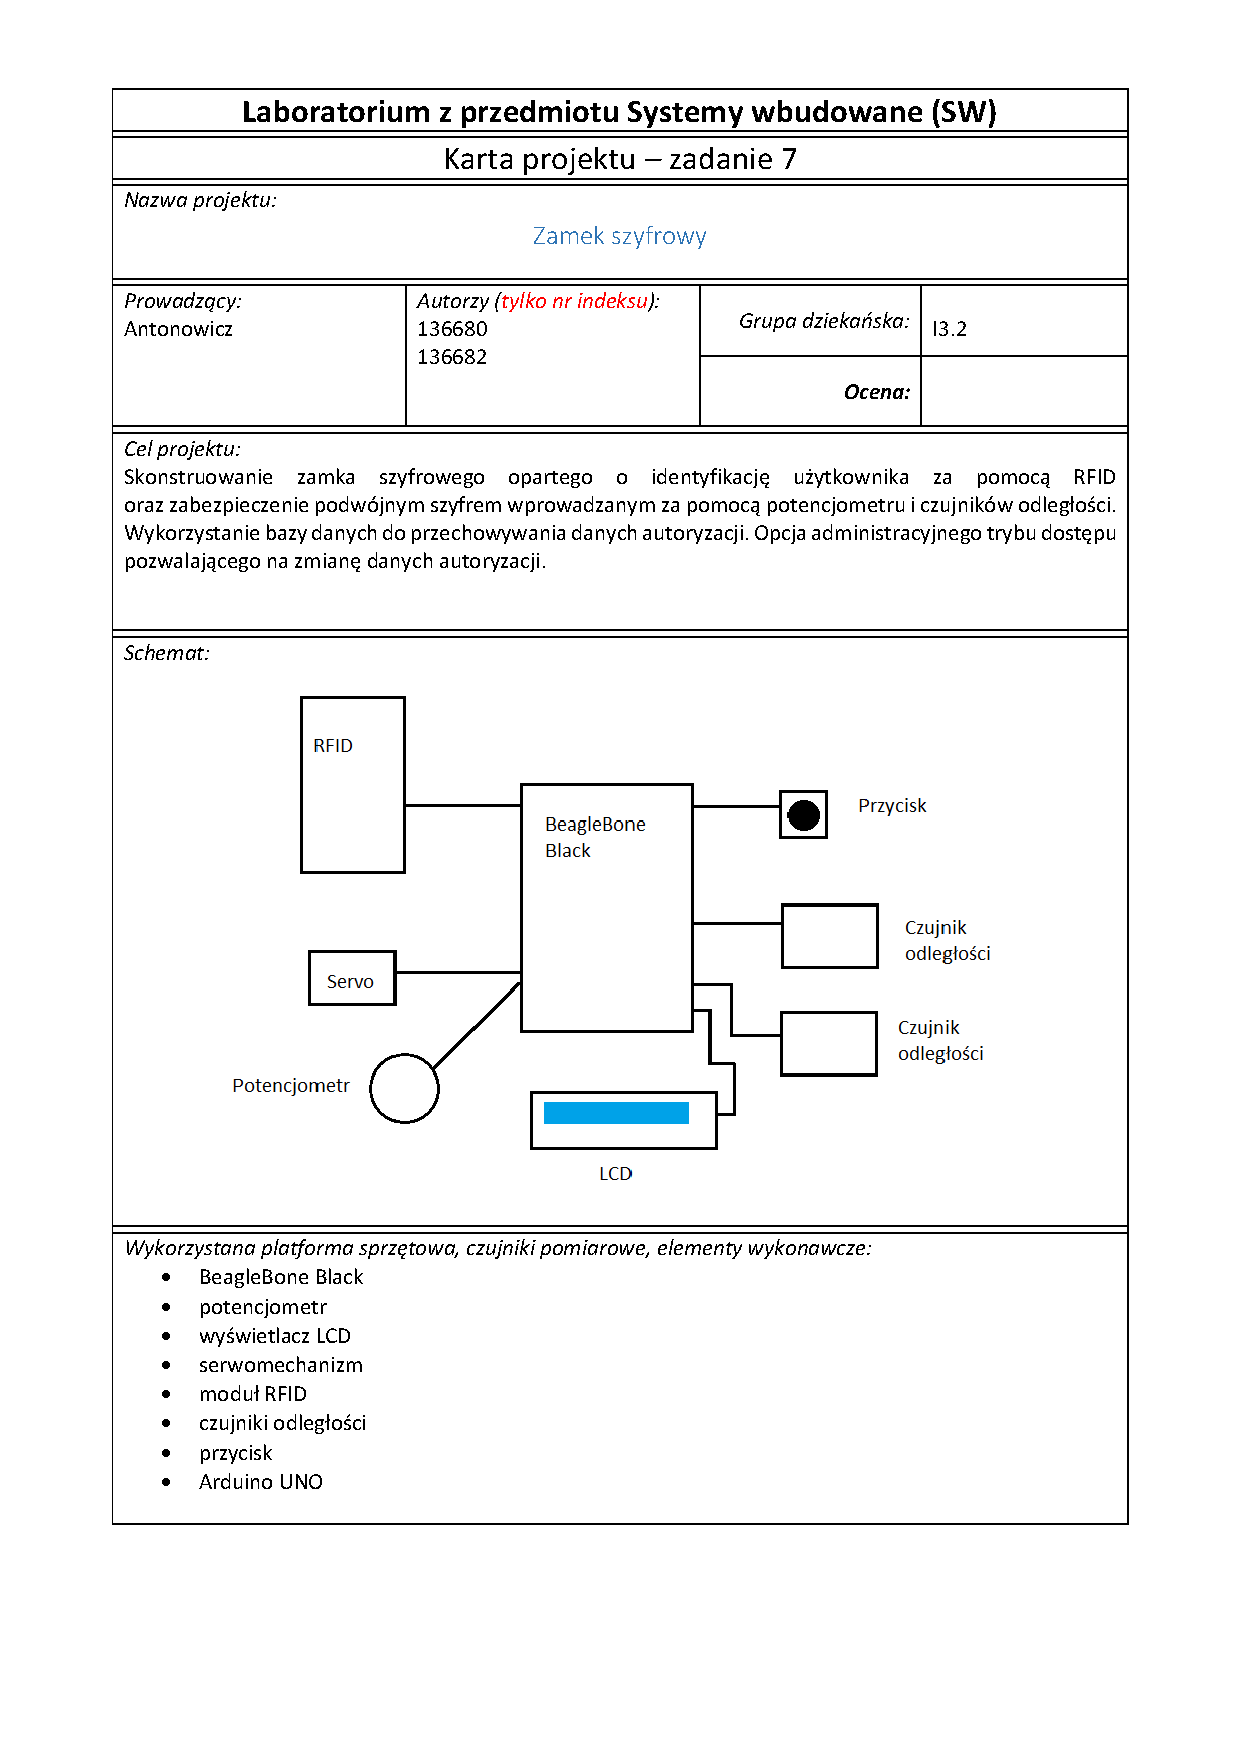
\includepdf{SW_KARTA_PROJ.pdf}
	
	\section{Zakres projektu}
	%TODO
	
	\section{Realizacja}
	%TODO: Schemat i zdjęcie całego układu z krótkim opisem
	
	\subsection{Interakcja z użytkownikiem}
	Interakcja systemu z użytkownikiem przebiega następująco:
	\begin{enumerate}
		\item Użytkownik identyfikuje się za pomocą prywatnego transpondera RFID.
		\item System weryfikuje użytkownika i wyświetla komunikat z żądaniem wprowadzenia szyfru podstawowego.
		\item Użytkownik wprowadza szyfr podstawowy za pomocą układu potencjometru.
		\item System sprawdza poprawność szyfru i wyświetla komunikat z żądaniem wprowadzenia szyfru drugorzędnego.
		\item Użytkownik wprowadza szyfr drugorzędny za pomocą układu czujników odległości.
		\item System sprawdza poprawność szyfru i otwiera zamek.
		\item Użytkownik zamyka zamek przez naciśnięcie przycisku.
	\end{enumerate}
	Możliwy jest również alternatywny scenariusz, w którym odebrany przez czytnik RFID identyfikator należy do administratora systemu:
	\begin{enumerate}
		\item Administrator identyfikuje się za pomocą transpondera RFID.
		\item System weryfikuje użytkownika i przełącza się w tryb administracyjny.
		\item System odczytuje za pomocą czytnika RFID identyfikator użytkownika, dla którego mają zostać wprowadzone nowe kody dostępu.
		\item System wyświetla komunikat z żądaniem utworzenia szyfru podstawowego.
		\item Użytkownik wprowadza nowy szyfr podstawowy za pomocą układu potencjometru.
		\item System wyświetla komunikat z żądaniem potwierdzenia nowego szyfru.
		\item Użytkownik ponownie wprowadza szyfr podstawowy z kroku 5.
		\item System sprawdza poprawność szyfru i wyświetla komunikat z żądaniem utworzenia szyfru drugorzędnego.
		\item Użytkownik wprowadza nowy szyfr drugorzędny za pomocą układu czujników odległości.
		\item System wyświetla komunikat z żądaniem potwierdzenia nowego szyfru.
		\item Użytkownik ponownie wprowadza szyfr podstawowy z kroku 9.
		\item System sprawdza poprawność szyfru i zapisuje nowe dane uwierzytelniania.
		\item System przełącza się w tryb podstawowy.
	\end{enumerate}
	Zmiana kodów dostępu jest również możliwa bez udziału administratora, jeśli zamek jest w danym momencie otwarty, a transponder użytkownika zostanie ponownie odczytany. W tym przypadku procedura zmiany danych uwierzytelniania przebiega zgodnie z punktami 3--12 scenariusza dostępu administracyjnego.
	
	\noindent\\
	Komunikaty systemu prezentowane są użytkownikowi za pomocą układu wyświetlacza LCD podłączonego do platformy Arduino UNO. Tekst do wyświetlenia jest przesyłany z programu głównego, uruchomionego na platformie BeagleBone Black, za pośrednictwem UART.
	
	\subsection{Identyfikacja użytkownika}
	Identyfikacja polega na odczycie przez czytnik RFID numeru UID transpondera użytkownika. Czytnik jest podłączony do platformy Arduino UNO. Po wykryciu transpondera następuje odczytanie numeru identyfikacyjnego i przesłanie go do programu głównego za pośrednictwem UART. Następnie wykonane zostaje zapytanie do bazy danych, które pozwala stwierdzić, czy użytkownik o danym UID jest zarejestrowany w systemie, a także czy posiada on status administratora.
	
	\subsection{Uwierzytelnianie}
	%TODO
	
	\subsection{Sterowanie zamkiem}
	%TODO
	
	\subsection{Sposób przechowywania danych}
	%TODO
	
	\section{Wnioski}
	%TODO
	
\end{document}
